
{\color{red} 

\section{Comparison of Full Run 1-9 vs. Run 1-9c Results}\label{app:compare_R1-9d_R1-9c}

\subsection{Comparison of Expected Sensitivities}\label{app:compare_sensitivity}

Figs \ref{fig:sensitivity_rate-only_Run1-9d_vs_Run1-9c} and \ref{fig:sensitivity_rate+shape_Run1-9d_vs_Run1-9c} show the expected Asimov A sensitivities compared between Run 1-9d and Run 1-9c for the rate-only and rate+shape analyses, respectively. For both analyses, the distributions have broadened and their separation has increased. A comparison of the p-values and test statistics is shown in Tab \ref{tab:sensitivity_comparison_rate_R19d_R17} for the rate-only analysis and for Tab \ref{tab:sensitivity_comparison_shape_R19d_R17} for the rate+shape analysis.

Compared to the Run 1-9c analysis, the Run 1-9d analysis expects a stronger exclusion of the $\beta=0$ hypothesis in both analyses. This is driven by the combination of two factors: 
\begin{enumerate}
	\item The increased statistics further separates the two distributions, as for $\beta=0$ it contains only background events while for $\beta=1$ it contains both signal and background events.
	
	\item The Asimov dataset assumes the $\beta=1$ hypothesis to be true and uses most probable values obtained by the Bayesian analysis on the T2K run 1-4 neutrino mode data \cite{T2KLongPaper}, so its test statistic value is close to the mean value of the $\beta=1$ distribution for each run period.
\end{enumerate}

Both the Run 1-9d and Run 1-9c analyses expect to disfavour the $\beta=1$ hypothesis at an approximately equal level due to the second point above. 


\subsection{Comparison of Data Results} \label{app:compare_data}

Figs \ref{fig:data_rate-only_Run1-9d_vs_Run1-9c} and \ref{fig:data_rate+shape_Run1-9d_vs_Run1-9c} show the observed distributions and test statistics compared between Run 1-9d and Run 1-9c for the rate-only and rate+shape analyses, respectively. A comparison of the p-values and test statistics is shown in Tab \ref{tab:data_comparison_rate_R19d_R17} for the rate-only analysis and for Tab \ref{tab:data_comparison_shape_R19d_R17} for the rate+shape analysis.

For both rate-only and rate+shape analyses, the $\beta=0$ ($\beta=1$) hypothesis is excluded at a greater (lesser) significance in the Run 1-9d analysis than in Run 1-9c. There are two reasons for this change. The first reason is shared by both rate-only and rate+shape analyses - the increased statistics further separates the two distributions (as explained in sec \ref{app:compare_sensitivity}). 

For the rate-only analysis the second reason is that the event rate has increased from $8.01 \frac{\text{events}}{10^{21} \text{POT}}$ in Run 1-9c to $9.18 \frac{\text{events}}{10^{21} \text{POT}}$ in Run 1-9d, shifting the rate-only test statistic closer to the mean value of the $\beta = 1$ distribution and further from the mean of the $\beta = 0$ distribution.

For the rate+shape analysis, the second reason for this change can be seen by comparing Fig \ref{fig:asimova_spectra_Run1-9d_RHC1Re} to Fig \ref{fig:asimova_spectra_RHC1Re}. It  can be seen that of the six newly collected (Run 9d) events in the antineutrino mode single-ring electron-like sample, five events are in the most likely region as predicted by the Asimov A dataset under the assumption of the $\beta = 1$ hypothesis. This is in contrast to the Run 1-9c data, where most of the nine events lay outside this region. This has the effect of changing the data $\Delta \chi^2$ value from the Run 1-9c value of \DeltachisqData\ to the Run 1-9d value of \DeltachisqDataRunOneNineD. This $\Delta \chi^2$ value is now close to the mean of the $\beta=1$ distribution, rather than almost midway between the two distributions, as was the case in Run 1-9c. This change is further demonstrated by the Bayes factor of \BayesFactorDataRunOneNineD\ which corresponds to a substantial preference for the $\beta = 1$ hypothesis over $\beta = 0$, while for the Run 1-9c analysis the Bayes factor was \BayesFactorData\, meaning a poor preference for the $\beta = 0$ hypothesis over $\beta = 1$.

\newpage


\begin{table}
	\centering
	\begin{tabular}{|c|c|c|c|c|c|c|}
		\hline
		\multirow{2}{*}{Run} & \multirow{2}{*}{RHC POT}   & \multirow{2}{*}{$N_{exp}$}    & \multicolumn{2}{|c|}{$\beta=0$} & \multicolumn{2}{|c|}{$\beta=1$} \\
		\cline{4-7}     				
		     		         &                            &   				 	          & p-value        & $\sigma$       & p-value      & $\sigma$         \\
		\hline
		
		
		1-9d                 & \TotalPotNuBarRunOneNine   & \NskOscExpectationNueBarRunOneNineD & \pvalRateOnlyBetaZeroAsimovARunOneNineD & \sigmaRateOnlyBetaZeroAsimovARunOneNineD & \pvalRateOnlyBetaOneAsimovARunOneNineD  & \sigmaRateOnlyBetaOneAsimovARunOneNineD \\
		\hline
		
		
		1-9c                 & \TotalPotNuBarRunOneNineC  & \NskOscExpectationNueBarRunOneNineC & \pvalRateOnlyBetaZeroAsimovA & \sigmaRateOnlyBetaZeroAsimovA & \pvalRateOnlyBetaOneAsimovA & \sigmaRateOnlyBetaOneAsimovA \\
		\hline
		
		
		1-7                  & \TotalPotNuBarRunOneSevenC & 6.008	  & $0.0511 \pm 0.00002$  & $1.9506 \pm 0.0002$		 & $0.5022 \pm 0.00005$   & $0.67103 \pm 0.0008$ \\
		\hline
	\end{tabular}
	\caption{Expected rate-only p-values and the number of events from the full Run 1-9 data set compared to the Run 1-9c and Run 1-7 data set used for previous iterations of this analysis, in Summer 2018 and 2016\cite{OurRun16AntiNueBarAppearanceAnalysis3Flavour}, respectively.}
	\label{tab:sensitivity_comparison_rate_R19d_R17}
\end{table}


\begin{table}
	\centering
	\begin{tabular}{|c|c|c|c|c|c|c|c|}
		\hline
		\multirow{2}{*}{Run} & \multirow{2}{*}{RHC POT} & \multirow{2}{*}{$\Delta \chi^2_{\textrm{exp}}$} & \multicolumn{2}{|c|}{$\beta=0$} & \multicolumn{2}{|c|}{$\beta=1$} & \multirow{2}{*}{$B_{01}$}\\
		\cline{4-7}      				
		                     &   				 	    &                                                 & p-value         & $\sigma$      & p-value         & $\sigma$      &   \\
		\hline
		
		
		1-9d                 & \TotalPotNuBarRunOneNine & \DeltachisqAsimovARunOneNineD                   & \pvalRateShapeBetaZeroAsimovARunOneNineD & \sigmaRateShapeBetaZeroAsimovARunOneNineD & \pvalRateShapeBetaOneAsimovARunOneNineD & \sigmaRateShapeBetaOneAsimovARunOneNineD & \BayesFactorAsimovARunOneNineD \\
		\hline
		
		
		1-9c                 & \TotalPotNuBarRunOneNineC& \DeltachisqAsimovA                              & \pvalRateShapeBetaZeroAsimovA & \sigmaRateShapeBetaZeroAsimovA & \pvalRateShapeBetaOneAsimovA & \sigmaRateShapeBetaOneAsimovA & \BayesFactorAsimovA \\
		\hline
		
		
		1-7                  &\TotalPotNuBarRunOneSevenC& 2.610			                                  & $0.043 \pm 0.002$ & $2.02 \pm 0.02$	  &  $0.444 \pm 0.005$ & $0.765 \pm 0.008$		  & 0.271 \\
		\hline
	\end{tabular}
	\caption{Expected rate+shape p-values, $\Delta \chi^2$ and Bayes factor from the full Run 1-9 data set compared to the Run 1-9c and Run 1-7 data set used for previous iterations of this analysis, in Summer 2018 and 2016\cite{OurRun16AntiNueBarAppearanceAnalysis3Flavour}, respectively.}
	\label{tab:sensitivity_comparison_shape_R19d_R17}
\end{table}

\begin{table}
	\centering
	\begin{tabular}{|c|c|c|c|c|c|c|}
		\hline
		\multirow{2}{*}{Run} & \multirow{2}{*}{RHC POT}   & \multirow{2}{*}{$N_{obs}$}    & \multicolumn{2}{|c|}{$\beta=0$} & \multicolumn{2}{|c|}{$\beta=1$} \\
		\cline{4-7}     				
		     		         &                            &   				 	          & p-value        & $\sigma$       & p-value      & $\sigma$         \\
		\hline
		
		
		1-9d                 & \TotalPotNuBarRunOneNine   & \NskObservedNueBarRunOneNineD & \pvalRateOnlyBetaZeroDataRunOneNineD & \sigmaRateOnlyBetaZeroDataRunOneNineD & \pvalRateOnlyBetaOneDataRunOneNineD  & \sigmaRateOnlyBetaOneDataRunOneNineD \\
		\hline
		
		
		1-9c                 & \TotalPotNuBarRunOneNineC  & \NskObservedNueBarRunOneNineC & \pvalRateOnlyBetaZeroData & \sigmaRateOnlyBetaZeroData & \pvalRateOnlyBetaOneData & \sigmaRateOnlyBetaOneData \\
		\hline
		
		
		1-7                  & \TotalPotNuBarRunOneSevenC & 4			  				  & $0.4100 \pm 0.00005$  & $0.8239 \pm 0.00009$			& $0.2155 \pm 0.00004$       & $1.2486 \pm 0.0001$ \\
		\hline
	\end{tabular}
	\caption{Observed rate-only p-values and number of events from the full Run 1-9 data set compared to the Run 1-9c and Run 1-7 data set used for previous iterations of this analysis, in Summer 2018 and 2016\cite{OurRun16AntiNueBarAppearanceAnalysis3Flavour}, respectively.}
	\label{tab:data_comparison_rate_R19d_R17}
\end{table}


\begin{table}
	\centering
	\begin{tabular}{|c|c|c|c|c|c|c|c|}
		\hline
		\multirow{2}{*}{Run} & \multirow{2}{*}{RHC POT} & \multirow{2}{*}{$\Delta \chi^2_{\textrm{obs}}$} & \multicolumn{2}{|c|}{$\beta=0$} & \multicolumn{2}{|c|}{$\beta=1$} & \multirow{2}{*}{$B_{01}$}\\
		\cline{4-7}      				
		                     &   				 	    &                                                 & p-value         & $\sigma$      & p-value         & $\sigma$      &   \\
		\hline
		
		
		1-9d                 & \TotalPotNuBarRunOneNine & \DeltachisqDataRunOneNineD                      & \pvalRateShapeBetaZeroDataRunOneNineD & \sigmaRateShapeBetaZeroDataRunOneNineD & \pvalRateShapeBetaOneDataRunOneNineD & \sigmaRateShapeBetaOneDataRunOneNineD & \BayesFactorDataRunOneNineD \\
		\hline
		
		
		1-9c                 & \TotalPotNuBarRunOneNineC& \DeltachisqData                                 & \pvalRateShapeBetaZeroData & \sigmaRateShapeBetaZeroData & \pvalRateShapeBetaOneData & \sigmaRateShapeBetaOneData & \BayesFactorData \\
		\hline
		
		
		1-7                  &\TotalPotNuBarRunOneSevenC& -1.930			                              & $0.3742 \pm 0.0048$			& $0.888 \pm 0.009$		    & $0.099 \pm 0.003$		      & $1.65 \pm 0.01$		  & 2.62 \\
		\hline
	\end{tabular}
	\caption{Observed rate+shape p-values, $\Delta \chi^2$ and Bayes factor from the full Run 1-9 data set compared to the Run 1-9c and Run 1-7 data set used for previous iterations of this analysis, in Summer 2018 and 2016\cite{OurRun16AntiNueBarAppearanceAnalysis3Flavour}, respectively.}
	\label{tab:data_comparison_shape_R19d_R17}
\end{table}


\begin{figure}
	\centering
	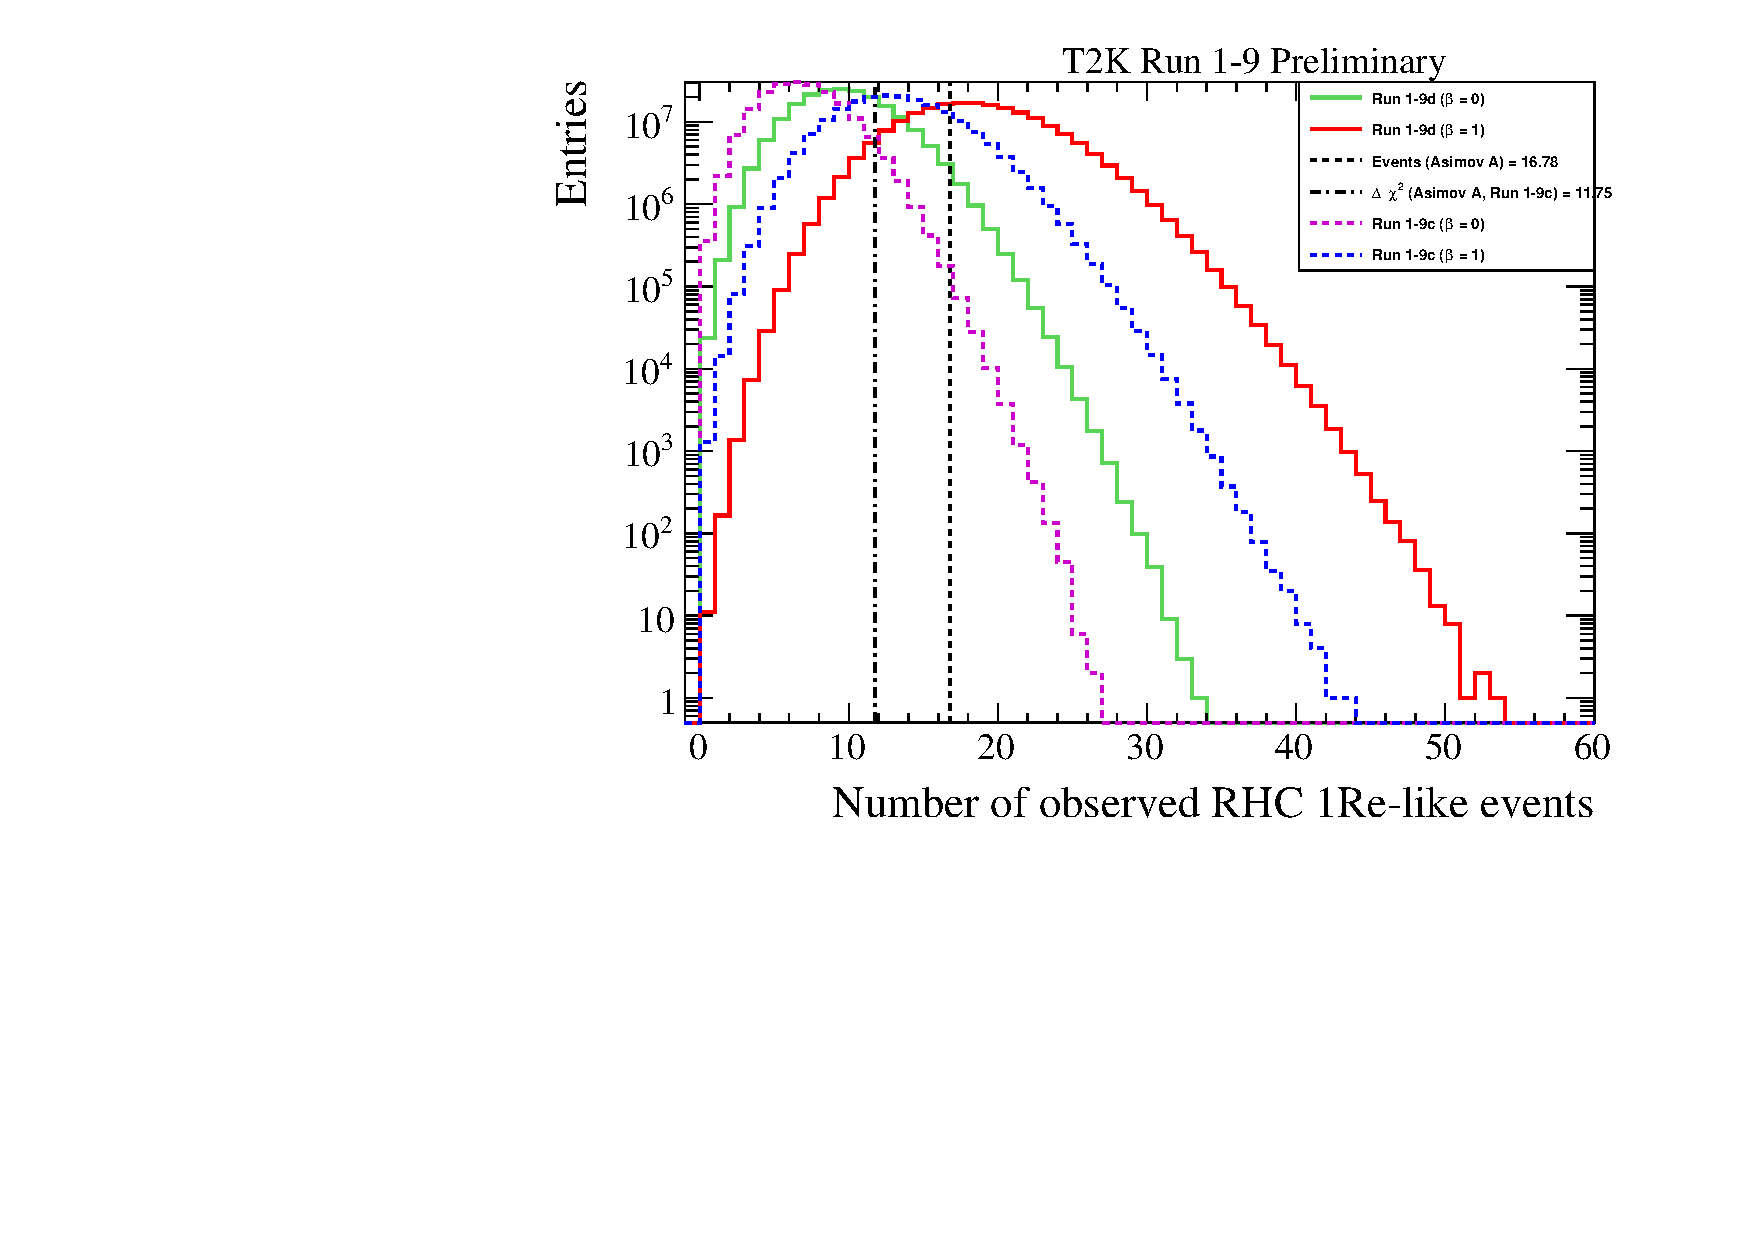
\includegraphics[scale=0.65]{sensitivity/compare_R1-9d_vs_R1-9c/nuebarapp_graphs_nmargtoys=200k_nexp=20k_rate-only_MCsampling_R19d_vs_R19c_comparison_nevents_log}
	\caption{Comparison between the expected Run 1-9d and Run 1-9c distributions of the total number of events in the antineutrino mode single-ring e-like sample. The distributions were produced with \NToysFakeDataRateOnly\ toy experiments for both the $\beta = 0$ and $\beta = 1$ hypotheses using the method outlined in section \ref{sec:method_rate-only} and the Asimov A spectra to calculate the 4-sample likelihood.}
	\label{fig:sensitivity_rate-only_Run1-9d_vs_Run1-9c}
\end{figure}

\begin{figure}
	\centering
	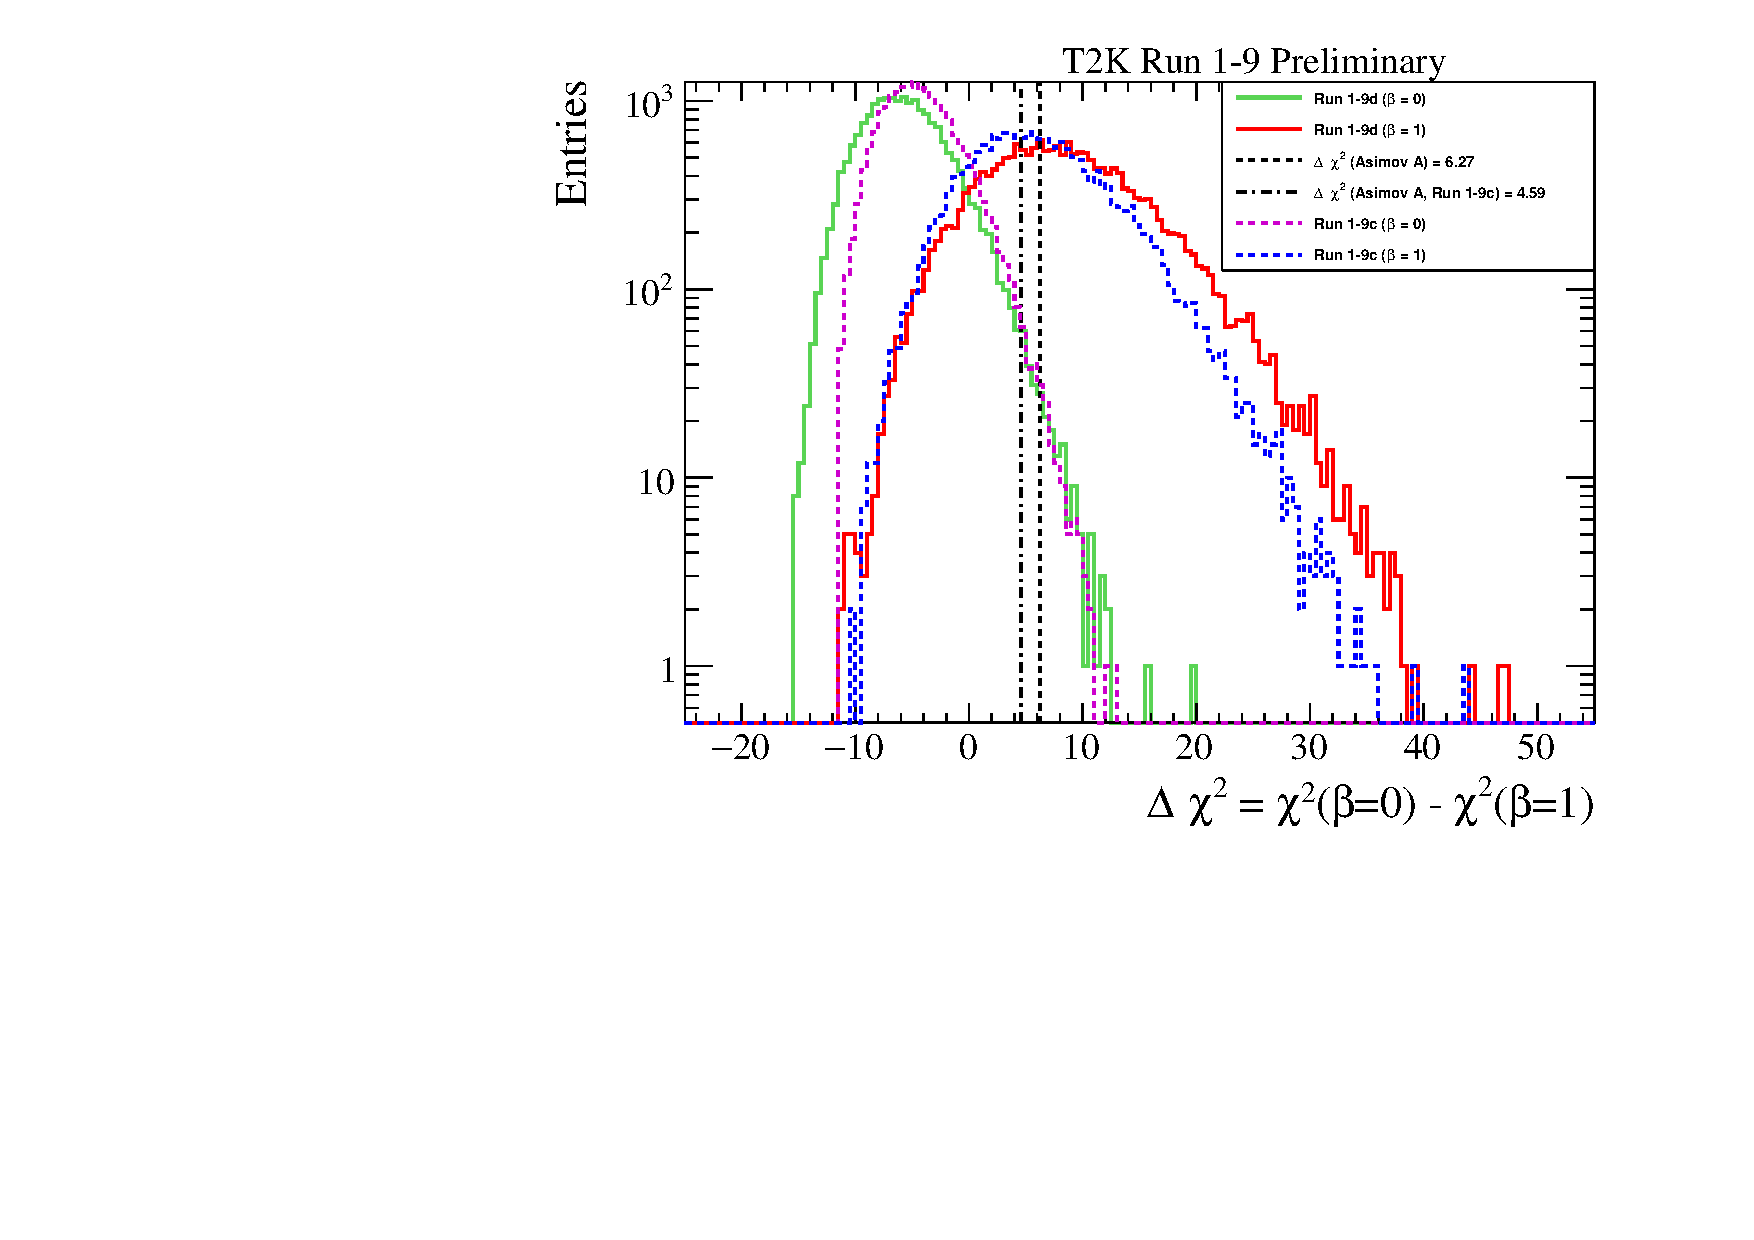
\includegraphics[scale=0.65]{sensitivity/compare_R1-9d_vs_R1-9c/nuebarapp_graphs_nmargtoys=200k_nexp=20k_rate+shape_R19d_vs_R19c_comparison_Deltachisq_log}
	\caption{Comparison between the expected Run 1-9d and Run 1-9c distributions of Asimov-constrained $\Delta \chi^2$ values. The distributions were produced with \NToysFakeDataRatePlusShape\ toy experiments for both the $\beta = 0$ and $\beta = 1$ hypotheses using the method outlined in section \ref{sec:method_rate+shape} with the Asimov A spectra to calculate the 4-sample likelihood.}
	\label{fig:sensitivity_rate+shape_Run1-9d_vs_Run1-9c}
\end{figure}


\begin{figure}
	\centering
	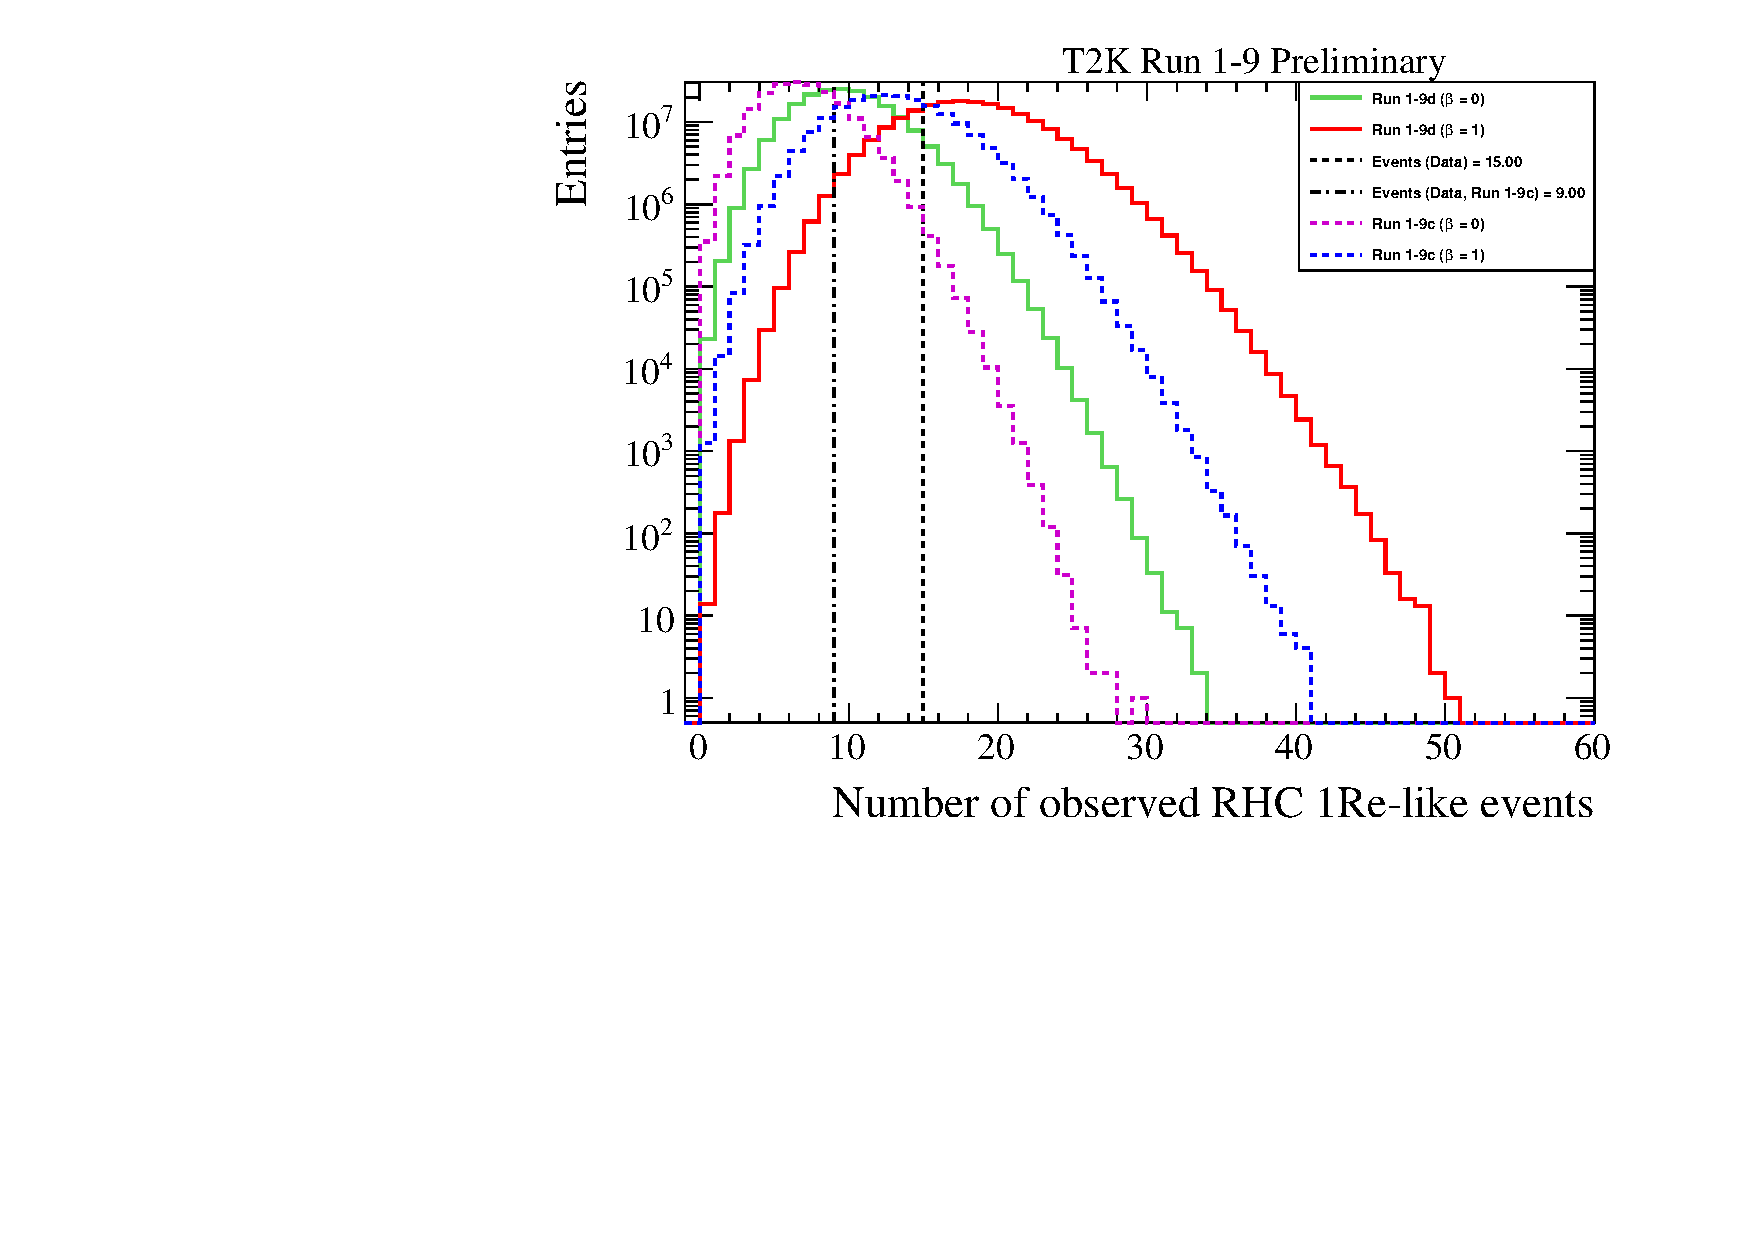
\includegraphics[scale=0.65]{data/compare_R1-9d_vs_R1-9c/nuebarapp_graphs_nmargtoys=200k_nexp=20k_rate-only_Run1-9d_vs_Run1-9c_comparison_nevents_log}
	\caption{Comparison between the observed Run 1-9d and Run 1-9c distributions of the total number of events in the antineutrino mode single-ring e-like sample. The distributions were produced with \NToysFakeDataRateOnly\ toy experiments for both the $\beta = 0$ and $\beta = 1$ hypotheses using the method outlined in section \ref{sec:method_rate-only} and the data spectra to calculate the 4-sample likelihood.}
	\label{fig:data_rate-only_Run1-9d_vs_Run1-9c}
\end{figure}

\begin{figure}
	\centering
	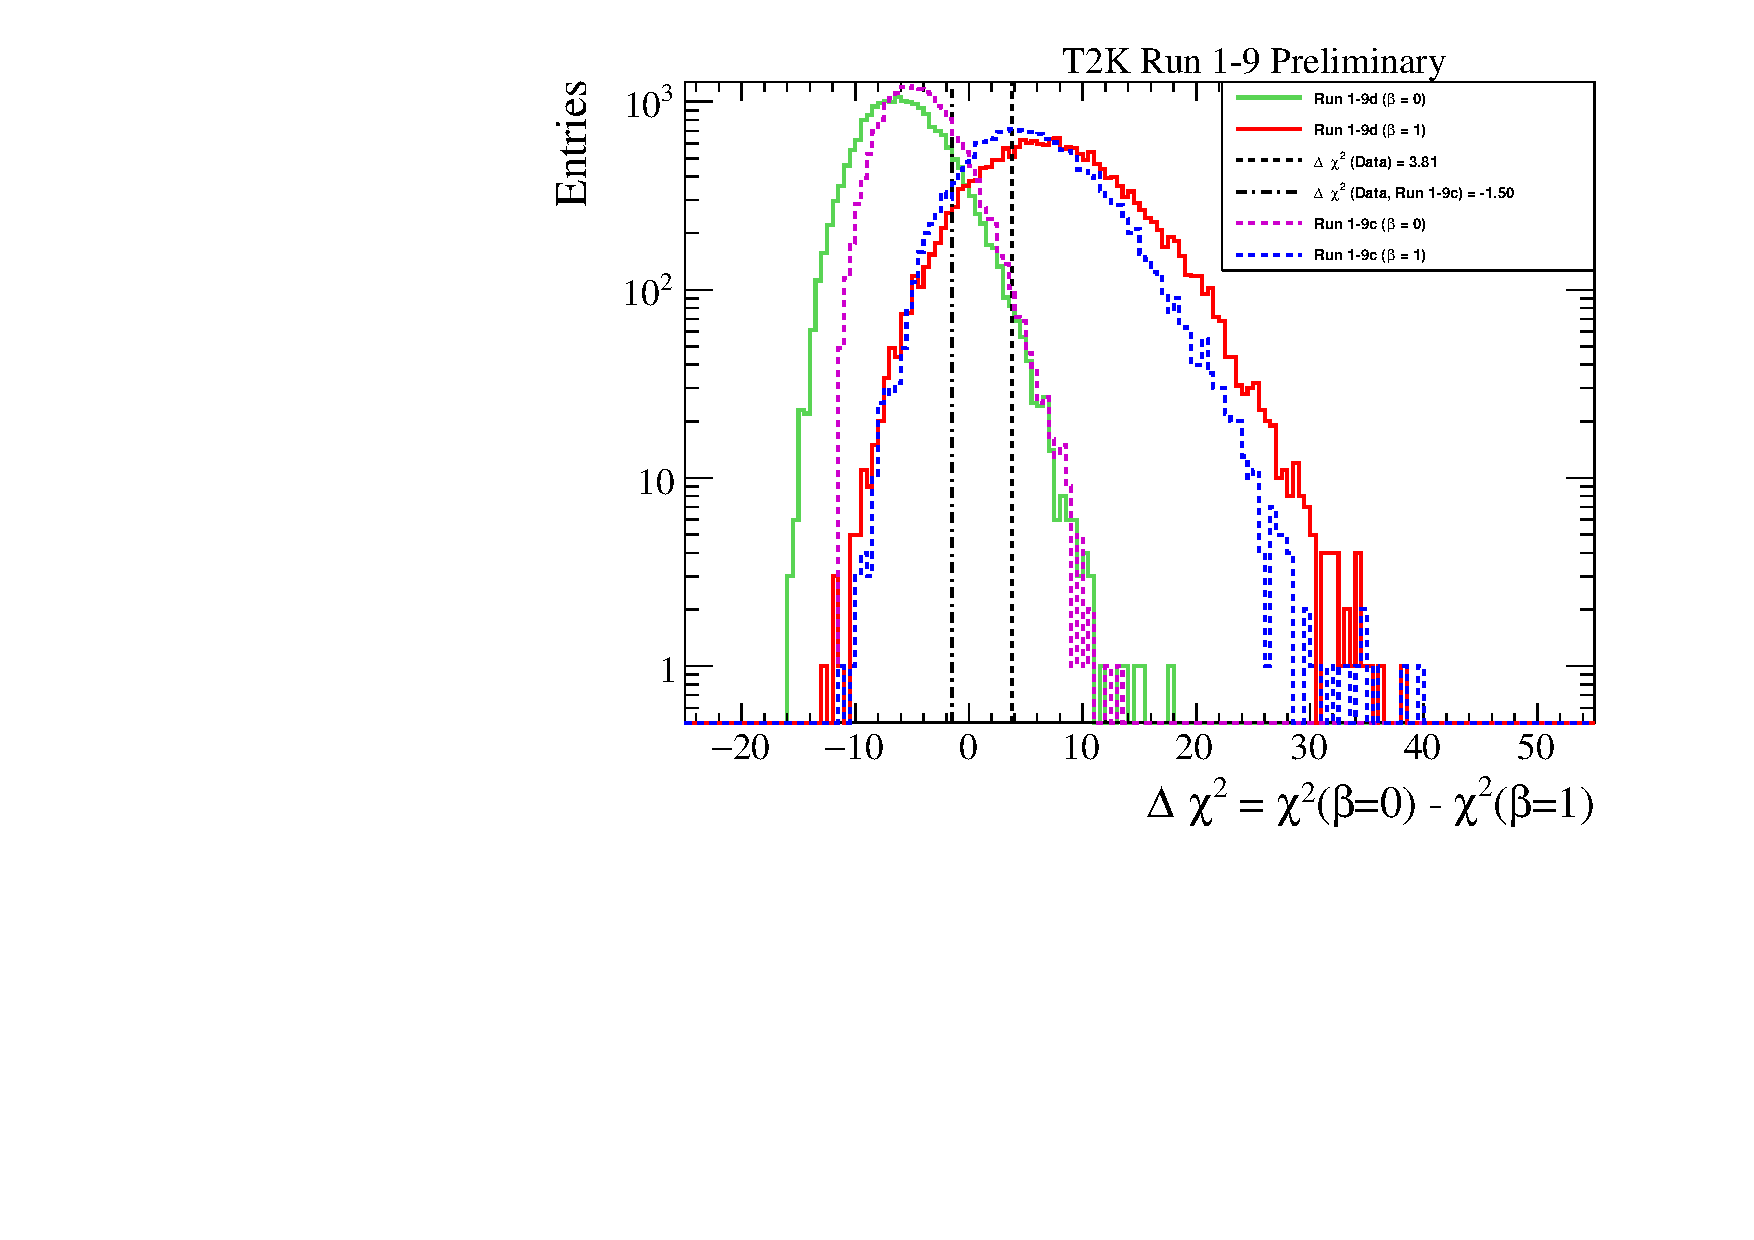
\includegraphics[scale=0.65]{data/compare_R1-9d_vs_R1-9c/nuebarapp_graphs_nmargtoys=200k_nexp=20k_rate+shape_Run1-9d_vs_Run1-9c_comparison_Deltachisq_log}
	\caption{Comparison between the observed Run 1-9d and Run 1-9c distributions of data-constrained $\Delta \chi^2$ values. The distributions were produced with \NToysFakeDataRatePlusShape\ toy experiments for both the $\beta = 0$ and $\beta = 1$ hypotheses using the method outlined in section \ref{sec:method_rate+shape} with the data spectra to calculate the 4-sample likelihood.}
	\label{fig:data_rate+shape_Run1-9d_vs_Run1-9c}
\end{figure}

} % \colour{red}

\FloatBarrier

